%% LyX 2.3.6.1 created this file.  For more info, see http://www.lyx.org/.
%% Do not edit unless you really know what you are doing.
\documentclass[twoside,twocolumn,english,aps,nofootinbib,superscriptaddress,notitlepage,longbibliography]{revtex4-2}
\usepackage[T1]{fontenc}
\usepackage{geometry}
\geometry{verbose}
\setcounter{secnumdepth}{2}
\setcounter{tocdepth}{2}
\usepackage{color}
\usepackage{amsmath}
\usepackage{amssymb}
\usepackage{graphicx}

\makeatletter
%%%%%%%%%%%%%%%%%%%%%%%%%%%%%% User specified LaTeX commands.
\usepackage{times}
\usepackage{tikz-feynman}
\usepackage{feynmf}
\usepackage{tabularx}
\usepackage{xfrac}
\usepackage{amsfonts}
\usepackage{longtable}
\usepackage{booktabs}\usepackage{url}
\usepackage{subfigure}
\usepackage{dsfont}
\usepackage{booktabs}
\usepackage{dcolumn}
\usepackage{amsthm}
\usepackage{bm}
\usepackage{multirow}
%\usepackage{cleveref}
\usepackage{mathrsfs}
\usepackage{amsfonts}
\usepackage{dcolumn}
\usepackage{bm}
\usepackage{multirow}
\usepackage{color}
\usepackage{extarrows}
\usepackage{datetime}
\usepackage{comment}
\usepackage[super]{nth}
\usepackage{braket}
\usepackage{tikz-network}

\def\Z{\mathbb{Z}}
\newcommand{\red}[1]{{\textcolor{red}{#1}}}
\newtheorem{theorem}{Theorem}\newtheorem{statement}{Statement}\newcommand{\mb}{\mathbb}
\newcommand{\bs}{\boldsymbol}
\newcommand{\wt}{\widetilde}
\newcommand{\mc}{\mathcal}
\newcommand{\ep}{\epsilon}
\newcommand{\tf}{\textbf}
\definecolor{myred}{RGB}{232,102,102}
\definecolor{myblue}{RGB}{187,187,255}
\definecolor{myorange0}{RGB}{252,226,5}
\definecolor{myorange0c}{RGB}{255,255,255}
\definecolor{myorange}{RGB}{255,165,0}
\definecolor{mygrey}{RGB}{105,105,105}
\definecolor{OliveGreen}{RGB}{85,107,47}
\definecolor{NavyBlue}{RGB}{0,0,128}
%\definecolor{myY}{RGB}{220,255,203}
\definecolor{mygreen}{RGB}{34,139,34}
\definecolor{myY}{RGB}{220,255,203}
\definecolor{myYO}{RGB}{255, 220, 151}

\definecolor{mygreenc}{RGB}{150,50,50}
\newcommand{\Wgatedagger}[2]{
\draw[very thick] (#1-0.5, #2 +0.5) -- (#1+0.5,#2-0.5);
\draw[very thick] (#1-0.5,#2-0.5) -- (#1+0.5,#2+0.5);
\draw[ thick, fill=mygreenc, rounded corners=2pt] (#1-0.25,#2+0.25) rectangle (#1+0.25,#2-0.25);
\draw[thick] (#1,#2+0.15) -- (#1+0.15,#2+0.15) -- (#1+0.15,#2);
%\Text[x=0,y=-0.075]{\x \y}
}
\newcommand{\Wgategreen}[2]{
\draw[very thick] (#1-0.5, #2 +0.5) -- (#1+0.5,#2-0.5);
\draw[very thick] (#1-0.5,#2-0.5) -- (#1+0.5,#2+0.5);
\draw[ thick, fill=mygreen, rounded corners=2pt] (#1-0.25,#2+0.25) rectangle (#1+0.25,#2-0.25);
\draw[thick] (#1,#2+0.15) -- (#1+0.15,#2+0.15) -- (#1+0.15,#2);
%\Text[x=0,y=-0.075]{\x \y}
}
\newcommand{\Wgatered}[2]{
\draw[very thick] (#1-0.5, #2 +0.5) -- (#1+0.5,#2-0.5);
\draw[very thick] (#1-0.5,#2-0.5) -- (#1+0.5,#2+0.5);
\draw[ thick, fill=myred, rounded corners=2pt] (#1-0.25,#2+0.25) rectangle (#1+0.25,#2-0.25);
\draw[thick] (#1,#2+0.15) -- (#1+0.15,#2+0.15) -- (#1+0.15,#2);
%\Text[x=0,y=-0.075]{\x \y}
}
\newcommand{\MYsquareB}[2]{

\draw[ thick, fill=black, rounded corners=2pt] (#1-0.25,#2+0.25) rectangle (#1+0.25,#2-0.25);
\draw[thick, color=white] (#1,#2+0.15) -- (#1+0.15,#2+0.15) -- (#1+0.15,#2);
%\Text[x=0,y=-0.075]{\x \y}
}
\newcommand{\Wgateblue}[2]{
\draw[very thick] (#1-0.5, #2 +0.5) -- (#1+0.5,#2-0.5);
\draw[very thick] (#1-0.5,#2-0.5) -- (#1+0.5,#2+0.5);
\draw[ thick, fill=myblue, rounded corners=2pt] (#1-0.25,#2+0.25) rectangle (#1+0.25,#2-0.25);
\draw[thick] (#1,#2+0.15) -- (#1+0.15,#2+0.15) -- (#1+0.15,#2);
%\Text[x=0,y=-0.075]{\x \y}
}
\newcommand{\MYcircle}[2]{
\draw[thick, fill=white] (#1,#2) circle (0.1cm); }
\newcommand{\MYsquare}[2]{
%\node[regular polygon,
%    draw= thick,
%    regular polygon sides = 4,
 %    fill =white,
 %    minimum size = .2cm
 %    ] (p) at (#1,#2) {}; 
 \coordinate (Origin) at (#1,#2);
\filldraw [thick, fill=white, even odd rule] ($(Origin)+(-.1cm,-.1cm)$) coordinate (Square) -- ++(0.0cm,0.2cm) -- ++(0.2cm,0.0cm) -- ++(0.0cm,-0.2cm) -- cycle;
 }
\newcommand{\MYtriangle}[2]{
 \coordinate (Origin) at (#1,#2);
\filldraw [thick, fill=white, even odd rule] ($(Origin)+(-.0cm,{0.666*cos(60)*0.3cm})$) coordinate (Triangle) -- ++(0.15cm,-{cos(60)*0.3cm}) -- ++(-0.3cm,0.0cm) -- ++(0.15cm,{cos(60)*0.3cm}) -- cycle;
}
\newcommand{\MYcircleB}[2]{
\draw[thick, fill=black] (#1,#2) circle (0.1cm); }

\newcommand{\rhoO}[2]{
\draw[very thick] (-.5+#1,0.5+#2) -- (#1,0+#2);
\draw[very thick] (#1,0+#2) -- (.5+#1,0.5+#2);
\draw[very thick] (-.5+#1,#2) -- (.5+#1,#2);
\draw[ thick, fill=mygreen, rounded corners=2pt] (-0.35+#1,0.2-0.25+#2) rectangle (0.35+#1,0.2+0.2+#2);
\draw[very thick] (0.1+#1,0.15+.18+#2)-- (.15+0.1+#1,0.15+.18+#2) -- (.15+0.1+#1,0+.18+#2);
}

\newcommand{\Wgategrey}[2]{
\draw[very thick] (#1-0.5, #2 +0.5) -- (#1+0.5,#2-0.5);
\draw[very thick] (#1-0.5,#2-0.5) -- (#1+0.5,#2+0.5);
\draw[ thick, fill=mygrey, rounded corners=2pt] (#1-0.25,#2+0.25) rectangle (#1+0.25,#2-0.25);
\draw[thick] (#1,#2+0.15) -- (#1+0.15,#2+0.15) -- (#1+0.15,#2);
%\Text[x=0,y=-0.075]{\x \y}
}
\newcommand{\mcirc}{\mathbin{\scalerel*{\fullmoon}{G}}}
\newcommand{\msquare}{\mathord{\scalerel*{\Box}{G}}}
\newcommand{\mcircf}{\mathbin{\scalerel*{\newmoon}{G}}}
\newcommand{\mtriangle}{\mathord{\scalerel*{\triangle}{G}}}

\newcommand{\tr}{\text{tr} \, }
\newcommand{\Tr}{\text{Tr} \, }
%Tiles
\newcommand{\lineW}{.8mm}
\newcommand{\sroot}{1.41421356237}

%\input{HeadIncludes.txt}
\def\scale{0.3}

\newcommand{\gs}[1]{{\color{red}[#1]}}
\newcommand{\pk}[1]{{\color{blue}#1}}

%Set up the metadata

\makeatother

\usepackage{babel}
\begin{document}

\section{Hierarchy Generalization of Dual Unitarity}

\subsection{Dual Unitary}

In this paper, we consider a chain of $L$ cells with each cell consisting
of $2$ sites characterized by local dimension $D$. Thus, the corresponding
total Hilbert space is $\mathcal{H}=(C^{D})^{2L}$. The local basis
vector is denoted by $\ket{j}$ with $j=0,1,\cdots,D-1$. The dynamics
of the chain is driven by brickwall floquet circuits\begin{equation*}
\begin{aligned}
& U_{\mathrm{floquet}}^{\dagger}aU_{\mathrm{floquet}}=\\
&
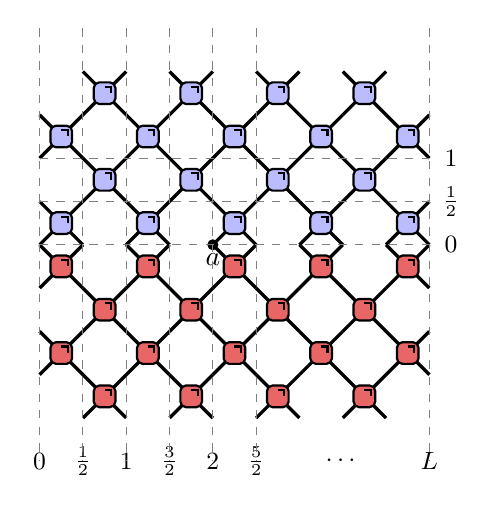
\begin{tikzpicture}[baseline=(current  bounding  box.center), scale=0.55]
\foreach \i in {0,...,4}
{
\foreach \j in {1,3}
{
\Wgatered{2*\i}{-\j+0.5}
\Wgateblue{2*\i}{\j-0.5}
}
}
\foreach \i in {0,...,3}
{
\foreach \j in {1,3}
{
\Wgatered{2*\i+1}{-\j-0.5}
\Wgateblue{2*\i+1}{\j+0.5}
}
}
\MYcircleB{3.5}{0}
\Text[x=3.5,y=-0.35]{$a$};
\foreach \i in {0,1,2}
{
\Text[x=2*\i-0.5,y=-5]{\small$\i$};
}
\foreach \i in {1,3,5}
{
\Text[x=\i-0.5,y=-5]{\small$\frac{\i}{2}$}
}
\Text[x=8.5,y=-5]{\small$L$};
\Text[x=6.5,y=-5]{\small$\cdots$};
\foreach \j in {0,1}
{
\Text[x=9,y=2*\j]{\small$\j$}
}
\foreach \j in {1}
{
\Text[x=9,y=\j]{\small$\frac{\j}{2}$}
}
\foreach \i in {0,1,2,3,4,5,9}
{
\draw[gray, dashed] (\i-0.5,5) -- (\i-0.5,-5);
}
\foreach \j in {0,1,2}
{
\draw[gray, dashed] (-0.5,\j) -- (8.5,\j);
}
\end{tikzpicture}
\end{aligned}
.
\end{equation*}Above, we graphically represented local unitary gates with dimension
$D^{2}\times D^{2}$ by a box with incoming and outgoing legs, \begin{equation}
U=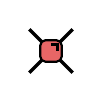
\begin{tikzpicture}[baseline=(current  bounding  box.center), scale=0.55]
\Wgatered{0}{0}
\end{tikzpicture}
,
\qquad
\qquad
U^{\dagger}=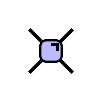
\begin{tikzpicture}[baseline=(current  bounding  box.center), scale=0.55]
\Wgateblue{5}{5}
\end{tikzpicture}.
\end{equation}The dual local gate $\tilde{U}$ is introduced by reshuffling the
indices
\begin{equation}
\bra{j}\bra{l}\tilde{U}\ket{i}\ket{k}=\bra{k}\bra{l}U\ket{i}\ket{j}.
\end{equation}
A gate is dual unitary (citations) means that not only $U$ is unitary
but also $\tilde{U}$, namely 
\begin{equation}
\tilde{U}^{\dagger}\tilde{U}=\tilde{U}\tilde{U}^{\dagger}=I_{D^{2}}\label{eq:algebric_dual_unitary}
\end{equation}
. It is easier to express our results in folded picture where $U^{\dagger}$
is folded back to $U$ to be a joint operator $U^{*}\otimes U$. We
use the empty bullet to represent the vectorized identity operator
in the folded picture as

\begin{equation}
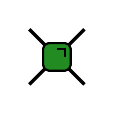
\begin{tikzpicture}[baseline=(current  bounding  box.center), scale=0.7]
\Wgategreen{0}{0}
\end{tikzpicture}
=
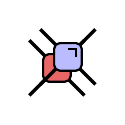
\begin{tikzpicture}[baseline=(current  bounding  box.center), scale=0.7]
\Wgatered{-0.1}{-0.1}
\Wgateblue{0.1}{0.1}
\end{tikzpicture}
,
\qquad
\qquad

\begin{tikzpicture}[baseline=(current  bounding  box.center), scale=0.7]
\MYcircle{0.25}{0.25}
\draw[very thick] (-0.25,-0.25)--(0.20,0.20);
\end{tikzpicture}
=

\begin{tikzpicture}[baseline=(current  bounding  box.center), scale=0.7]
\draw[very thick] (-0.25,-0.25)--(0.25,0.25)--(0.05,0.45)--(-0.45,-0.05);
\end{tikzpicture}
.
\end{equation} The unitarity condition reads as $
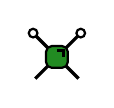
\begin{tikzpicture}[baseline=(current  bounding  box.center), scale=0.55]
\Wgategreen{0}{0}
\MYcircle{0.55}{0.55}
\MYcircle{-0.55}{0.55}
\end{tikzpicture}
=
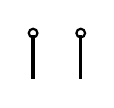
\begin{tikzpicture}[baseline=(current  bounding  box.center), scale=0.55]
\MYcircle{0.55}{0.55}
\MYcircle{-0.55}{0.55}
\draw[very thick] (-0.55,-0.5) -- (-0.55,0.5);
\draw[very thick] (0.55,-0.5) -- (0.55,0.5);
\end{tikzpicture}
$ and $
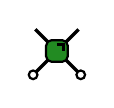
\begin{tikzpicture}[baseline=(current  bounding  box.center), scale=0.55]
\Wgategreen{0}{0}
\MYcircle{0.55}{-0.55}
\MYcircle{-0.55}{-0.55}
\end{tikzpicture}
=
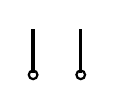
\begin{tikzpicture}[baseline=(current  bounding  box.center), scale=0.55]
\MYcircle{0.55}{-0.55}
\MYcircle{-0.55}{-0.55}
\draw[very thick] (-0.55,-0.5) -- (-0.55,0.5);
\draw[very thick] (0.55,-0.5) -- (0.55,0.5);
\end{tikzpicture}
$. The dual unitary condition (\ref{eq:algebric_dual_unitary}) can
be re-expressed in folded picture as

\begin{equation}
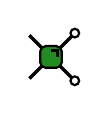
\begin{tikzpicture}[baseline=(current  bounding  box.center), scale=0.55]
\Wgategreen{0}{0}
\MYcircle{0.55}{0.55}
\MYcircle{0.55}{-0.55}
\end{tikzpicture}
=
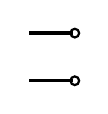
\begin{tikzpicture}[baseline=(current  bounding  box.center), scale=0.55]
\MYcircle{0.55}{0.55}
\MYcircle{0.55}{-0.55}
\draw[very thick] (-0.5,0.55) -- (0.5,0.55);
\draw[very thick] (-0.5,-0.55) -- (0.5,-0.55);
\end{tikzpicture}
;
\qquad
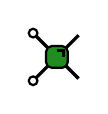
\begin{tikzpicture}[baseline=(current  bounding  box.center), scale=0.55]
\Wgategreen{0}{0}
\MYcircle{-0.55}{0.55}
\MYcircle{-0.55}{-0.55}
\end{tikzpicture}
=
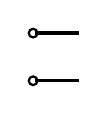
\begin{tikzpicture}[baseline=(current  bounding  box.center), scale=0.55]
\MYcircle{-0.55}{0.55}
\MYcircle{-0.55}{-0.55}
\draw[very thick] (-0.5,0.55) -- (0.5,0.55);
\draw[very thick] (-0.5,-0.55) -- (0.5,-0.55);
\end{tikzpicture}
. \label{eq:figure_dual_unitary_condi}
\end{equation}

This class of gates covers both integrable regions and chaotic regions
(citation). The parametrization of dual unitary gates when $D=2$
has been fully determined (citation). Although there is no complete
parametrization for dual unitary when $D\geq3$, some families of
the gates have been proposed (citation). In the following, we propose
a new parametrization of the $2-$qudit gates which can lead to a
large family of dual unitary gates in higher dimensions. This parametrization
method is also useful when we discuss the hierarchy generalization
of dual unitary circuits.

\subsection{Hierarchy Generalization}

The dual unitary circuit contributes an important and rare exactly
solvable model in understanding OTOC, quantum quench and many-body
phase transition(citation). A natural question is, whether the dual
unitarity condition is necessary in deriving this property. Another
motivation is that, some basic and famous Clifford gates, such as
Identity and Controlled-Not gate are not dual-unitary although they
are solvable. To address these problems, we generalize the definition
of dual unitary gate to a larger series so called as ``Hierarchy
Dual gate''. 

Since only one green box is involved in the dual-unitary condition
(\ref{eq:figure_dual_unitary_condi}), we call it as the $1_{\mathrm{st}}$
Hierarchy dual. In the next subsections \ref{subsec:Second-Hierarchy}
and \ref{subsec:Third-Hierarchy}, we generalize the dual unitary
($1_{\mathrm{st}}$ Hierarchy dual) to the $2_{\mathrm{nd}}$ and
$3_{\mathrm{rd}}$ Hierarchy dual and further study their parametrizations.

\subsection{Second Hierarchy\label{subsec:Second-Hierarchy}}

It is not necessary to simplify the quantum circuits. Indeed, we can
have a weaker condition

\begin{equation}
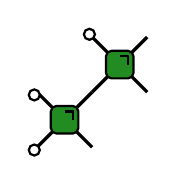
\begin{tikzpicture}[baseline=(current  bounding  box.center), scale=0.7]
\Wgategreen{0.5}{0.5}
\Wgategreen{-0.5}{-0.5}
\MYcircle{-0.05}{1.05}
\MYcircle{-1.05}{-0.05}
\MYcircle{-1.05}{-1.05}
\end{tikzpicture}
=
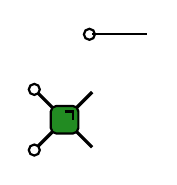
\begin{tikzpicture}[baseline=(current  bounding  box.center), scale=0.7]
\Wgategreen{-0.5}{-0.5}
\MYcircle{-0.05}{1.05}
\MYcircle{-1.05}{0.05}
\MYcircle{-1.05}{-1.05}
\draw[thick] (0,1.05)--(1,1.05);
\end{tikzpicture}
,
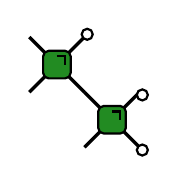
\begin{tikzpicture}[baseline=(current  bounding  box.center), scale=0.7]
\Wgategreen{-0.5}{0.5}
\Wgategreen{0.5}{-0.5}
\MYcircle{0.05}{1.05}
\MYcircle{1.05}{-0.05}
\MYcircle{1.05}{-1.05}
\end{tikzpicture}
=
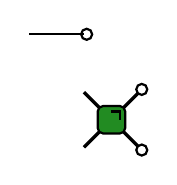
\begin{tikzpicture}[baseline=(current  bounding  box.center), scale=0.7]
\Wgategreen{0.5}{-0.5}
\MYcircle{0.05}{1.05}
\MYcircle{1.05}{0.05}
\MYcircle{1.05}{-1.05}
\draw[thick] (0,1.05)--(-1,1.05);
\end{tikzpicture}
\label{eq2:bottomtotop}
\end{equation}

Since this condition involves two green boxes on the left hand side,
we call it as the $2_{\mathrm{nd}}$ Hierarchy dual. It is remarkable
that the basic Clifford gates like Controlled-Not and Identity is
not dual unitary but instead $2_{\mathrm{nd}}$ Hierarchy dual. 

Algebraically, we can express the condition Eq. (\ref{eq2:bottomtotop})
as 
\begin{equation}
\begin{aligned}(I_{D}\otimes\tilde{U}^{\dagger})\cdot\tilde{U}^{\dagger}\tilde{U}\otimes I_{D}\cdot(I_{D}\otimes\tilde{U})=I_{D}\otimes\tilde{U}^{\dagger}\tilde{U},\\
(I_{D}\otimes\tilde{U})\cdot\tilde{U}\tilde{U}^{\dagger}\otimes I_{D}\cdot(I_{D}\otimes\tilde{U}^{\dagger})=I_{D}\otimes\tilde{U}\tilde{U}^{\dagger}.
\end{aligned}
\label{eq:2ndEq}
\end{equation}
A simple observation shows that if a circuit is $1_{\mathrm{st}}$
Hierarchy dual, it must be $2_{\mathrm{nd}}$ Hierarchy dual, therefore
$1_{\mathrm{st}}\subsetneqq2_{\mathrm{nd}}$. In this article, we
are interested in the gate which is only $2_{\mathrm{nd}}$ Hierarchy
dual but not first, denoting by $\overline{2}_{\mathrm{nd}}=2_{\mathrm{nd}}-1_{\mathrm{st}}$.
Similarly as in the $1_{\mathrm{st}}$ Hierarchy dual case (citation),
the full parametrization for qubit case is obtained as when $D=2$,
we have a nice parametrization of all interacting 2-qubit gate
\begin{equation}
U=v_{1}\otimes v_{2}e^{i(J_{x}\sigma_{x}\sigma_{x}+J_{y}\sigma_{y}\sigma_{y}+J_{z}\sigma_{z}\sigma_{z})}v_{3}\otimes v_{4}.
\end{equation}
Here $v_{1},v_{2},v_{3},v_{4}\in\mathbb{SU}(2)$ are all single site
gates. Due to the structure of gate, we can put $v_{3}=v_{4}=I_{D}$
without loss of generality since $v_{1}$ at this time step is always
combined with $v_{4}$ from the next time step therefore a redefinition
$v_{1}\to v_{4}\cdot v_{1}$ is always possible. The same argument
holds for $v_{2}$ and $v_{3}$. The $\overline{2}_{\mathrm{nd}}$
condition is that $J_{z}=\frac{\pi}{4},J_{x}=J_{y}=0$ and $v_{1},v_{2}\in\{U(r,\theta,\phi)|\sqrt{2}\sin r\sin\theta=\pm1\}$,
where $U(r,\theta,\phi)=e^{ir(\cos\theta\sigma_{z}+\sin\theta\cos\phi\sigma_{x}+\sin\theta\sin\phi\sigma_{y})}$
is the representation of $\mathbb{SU}(2)$ using Bloch sphere. Geometrically,
this particular combination of $r,\theta,\phi$ is a rotation which
rotates $\sigma_{z}$ to the $x-y$ plane.

In higher dimensions, though we don't have a complete parametrization
for $2_{\mathrm{nd}}$ Hierarchy dual, but we can still obtain two
rich families of $2_{\mathrm{nd}}$ Hierarchy dual. One is with generalized
Controlled-NOT gate in higher dimension defined as 
\begin{equation}
S=\sum_{i}\ket{i}\bra{i}\otimes X^{i},
\end{equation}
where $X$ is just the generator of Clifford gate in higher dimension.
As before, we can also put single site operator $v_{1}$ and $v_{2}$
at the top of $S$ subject to the constraint
\begin{equation}
\begin{aligned}\sum_{j}\bra{j}v_{1}\ket{i}\bra{j+k'-k}v_{1}^{*}\ket{i} & =\delta_{k,k'}\ \mathrm{for}\ \forall k,k',i.\\
\sum_{j}\bra{i}v_{2}\ket{j}\bra{i}v_{2}^{*}\ket{j+k'-k} & =\delta_{k,k'}\ \mathrm{for}\ \forall k,k',i.
\end{aligned}
\end{equation}
This two equations has a symmetry of transpose between each other. 

The other family is used the Clifford group method we developed in
the previous subsection(\textcolor{blue}{maybe a hyperlink in the
future}). With the proposed ansatz, we can simplify Eq. (\ref{eq:2ndEq})
to 
\begin{widetext}
\begin{equation}
\begin{aligned}(\sum_{b}\theta_{p_{b},q_{b}}^{*}\theta_{p_{b}+k,q_{b}+l})(\sum_{d}\theta_{p_{d},q_{d}}^{*}\theta_{p_{d}+s,q_{d}+t}M_{p_{d},q_{d}}^{\dagger}v_{1}^{*}M_{k,-l}v_{1}^{T}M_{p_{d},q_{d}})=0\ \forall(s,t)\neq(0,0)\ \mathrm{and}\ (k,l)\neq(0,0)\\
(\sum_{b}\theta_{p_{b},q_{b}}^{*}\theta_{p_{b}+k,q_{b}+l})(\sum_{d}\theta_{p_{d},q_{d}}^{*}\theta_{p_{d}+s,q_{d}+t}M_{-p_{d},q_{d}}^{\dagger}v_{2}^{*}M_{-k,-l}v_{2}^{T}M_{-p_{d},q_{d}})=0\ \forall(s,t)\neq(0,0)\ \mathrm{and}\ (k,l)\neq(0,0)
\end{aligned}
\end{equation}
\end{widetext}

If for $\forall(k,l)\neq(0,0)$, the first terms all vanish, this
will give the $1_{\mathrm{st}}$Hierarchy dual. Solving this nonlinear
equations we can get a family of solutions. For example, when $D=4k+2$
for some integer $k$, $\theta_{p,q}=\omega^{\frac{D}{2}pq}$ with
$v_{1}=v_{2}=I_{D}$ is a case for $\overline{2}_{\mathrm{nd}}$.
Also, $\theta_{p,q}=\begin{cases}
\omega^{\frac{p^{2}}{2}} & D=\mathrm{even}\\
\omega^{p^{2}} & D=\mathrm{odd}
\end{cases}$ is also $\overline{2}_{\mathrm{nd}}$ for some nontrivial $v_{1}$
and $v_{2}$.

Before ending this subsection, we point out that Eq. (\ref{eq2:bottomtotop})
also implies

\begin{equation}
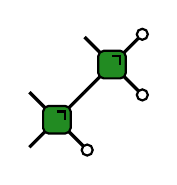
\begin{tikzpicture}[baseline=(current  bounding  box.center), scale=0.7]
\Wgategreen{-0.5}{-0.5}
\Wgategreen{0.5}{0.5}
\MYcircle{1.05}{1.05}
\MYcircle{1.05}{-0.05}
\MYcircle{0.05}{-1.05}
\end{tikzpicture}
=
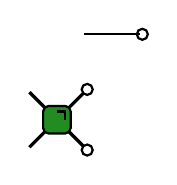
\begin{tikzpicture}[baseline=(current  bounding  box.center), scale=0.7]
\Wgategreen{-0.5}{-0.5}
\MYcircle{1.05}{1.05}
\MYcircle{0.05}{0.05}
\MYcircle{0.05}{-1.05}
\draw[thick] (0,1.05)--(1,1.05);
\end{tikzpicture}
,
\qquad
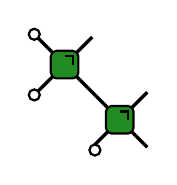
\begin{tikzpicture}[baseline=(current  bounding  box.center), scale=0.7]
\Wgategreen{-0.5}{0.5}
\Wgategreen{0.5}{-0.5}
\MYcircle{-1.05}{1.05}
\MYcircle{-1.05}{-0.05}
\MYcircle{0.05}{-1.05}
\end{tikzpicture}
=
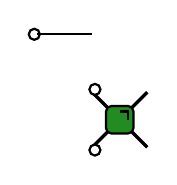
\begin{tikzpicture}[baseline=(current  bounding  box.center), scale=0.7]
\Wgategreen{0.5}{-0.5}
\MYcircle{-1.05}{1.05}
\MYcircle{0.05}{0.05}
\MYcircle{0.05}{-1.05}
\draw[thick] (0,1.05)--(-1,1.05);
\end{tikzpicture}
.
\label{eq:2ndfig}
\end{equation}

The prove strategy is by defining \begin{equation}
A=
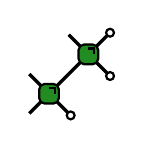
\begin{tikzpicture}[baseline=(current  bounding  box.center), scale=0.5]
\Wgategreen{-0.5}{-0.5}
\Wgategreen{0.5}{0.5}
\MYcircle{1.05}{1.05}
\MYcircle{1.05}{-0.05}
\MYcircle{0.05}{-1.05}
\end{tikzpicture}
-
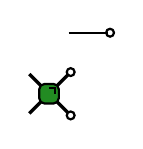
\begin{tikzpicture}[baseline=(current  bounding  box.center), scale=0.5]
\Wgategreen{-0.5}{-0.5}
\MYcircle{1.05}{1.05}
\MYcircle{0.05}{0.05}
\MYcircle{0.05}{-1.05}
\draw[thick] (0,1.05)--(1,1.05);
\end{tikzpicture}
,
B=
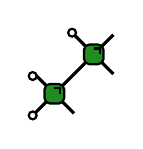
\begin{tikzpicture}[baseline=(current  bounding  box.center), scale=0.5]
\Wgategreen{-0.5}{-0.5}
\Wgategreen{0.5}{0.5}
\MYcircle{-0.05}{1.05}
\MYcircle{-1.05}{-0.05}
\MYcircle{-1.05}{-1.05}
\end{tikzpicture}
-
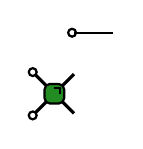
\begin{tikzpicture}[baseline=(current  bounding  box.center), scale=0.5]
\Wgategreen{-0.5}{-0.5}
\MYcircle{-0.05}{1.05}
\MYcircle{-1.05}{0.05}
\MYcircle{-1.05}{-1.05}
\draw[thick] (0,1.05)--(1,1.05);
\end{tikzpicture}
.
\end{equation}and we can prove $\mathrm{Tr}A^{\dagger}A=\mathrm{Tr}B^{\dagger}B$,
therefore the vanishing of $A$ also implies vanishing of $B$. This
can be proved graphically. To this end, we can introduce a four-folded
gate as $
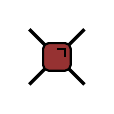
\begin{tikzpicture}[baseline=(current  bounding  box.center), scale=0.7]
\Wgatedagger{0}{0}
\end{tikzpicture}
=
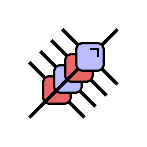
\begin{tikzpicture}[baseline=(current  bounding  box.center), scale=0.7]
\Wgatered{-0.3}{-0.3}
\Wgateblue{-0.1}{-0.1}
\Wgatered{0.1}{0.1}
\Wgateblue{0.3}{0.3}
\end{tikzpicture}
.
$The first term of $\mathrm{Tr}A^{\dagger}A$ is

\begin{equation}
\mathrm{Tr}
(
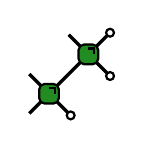
\begin{tikzpicture}[baseline=(current  bounding  box.center), scale=0.5]
\Wgategreen{-0.5}{-0.5}
\Wgategreen{0.5}{0.5}
\MYcircle{1.05}{1.05}
\MYcircle{1.05}{-0.05}
\MYcircle{0.05}{-1.05}
\end{tikzpicture}
)^{\dagger}
(
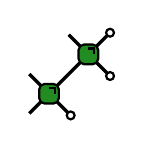
\begin{tikzpicture}[baseline=(current  bounding  box.center), scale=0.5]
\Wgategreen{-0.5}{-0.5}
\Wgategreen{0.5}{0.5}
\MYcircle{1.05}{1.05}
\MYcircle{1.05}{-0.05}
\MYcircle{0.05}{-1.05}
\end{tikzpicture}
)
=
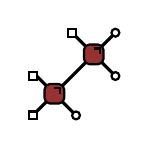
\begin{tikzpicture}[baseline=(current  bounding  box.center), scale=0.5]
\Wgatedagger{-0.5}{-0.5}
\Wgatedagger{0.5}{0.5}
\MYcircle{1.05}{1.05}
\MYcircle{1.05}{-0.05}
\MYcircle{0.05}{-1.05}
\MYsquare{-0.05}{1.05}
\MYsquare{-1.05}{-0.05}
\MYsquare{-1.05}{-1.05}
\end{tikzpicture}
,
\end{equation}where 
\begin{tikzpicture}[baseline=(current  bounding  box.center), scale=0.7]
\MYcircle{0.25}{0.25}
\draw[very thick] (-0.25,-0.25)--(0.20,0.20);
\end{tikzpicture} stands for the contraction between the same leg from the first and
second layer as well as the third and forth layer while 
\begin{tikzpicture}[baseline=(current  bounding  box.center), scale=0.7]
\MYsquare{0.25}{0.25}
\draw[very thick] (-0.25,-0.25)--(0.20,0.20);
\end{tikzpicture} stands for the contraction between the first and forth layer as well
as second and third layer. The result will be the same if we exchange
the second and forth layer, while simultaneously exchange 
\begin{tikzpicture}[baseline=(current  bounding  box.center), scale=0.7]
\MYcircle{0.25}{0.25}
\draw[very thick] (-0.25,-0.25)--(0.20,0.20);
\end{tikzpicture} and 
\begin{tikzpicture}[baseline=(current  bounding  box.center), scale=0.7]
\MYsquare{0.25}{0.25}
\draw[very thick] (-0.25,-0.25)--(0.20,0.20);
\end{tikzpicture}. Therefore, we arrive at\begin{equation}
\mathrm{Tr}
(
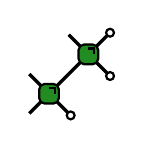
\begin{tikzpicture}[baseline=(current  bounding  box.center), scale=0.5]
\Wgategreen{-0.5}{-0.5}
\Wgategreen{0.5}{0.5}
\MYcircle{1.05}{1.05}
\MYcircle{1.05}{-0.05}
\MYcircle{0.05}{-1.05}
\end{tikzpicture}
)^{\dagger}
(
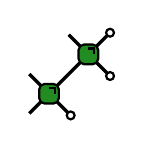
\begin{tikzpicture}[baseline=(current  bounding  box.center), scale=0.5]
\Wgategreen{-0.5}{-0.5}
\Wgategreen{0.5}{0.5}
\MYcircle{1.05}{1.05}
\MYcircle{1.05}{-0.05}
\MYcircle{0.05}{-1.05}
\end{tikzpicture}
)
=
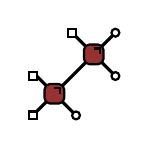
\begin{tikzpicture}[baseline=(current  bounding  box.center), scale=0.5]
\Wgatedagger{-0.5}{-0.5}
\Wgatedagger{0.5}{0.5}
\MYcircle{1.05}{1.05}
\MYcircle{1.05}{-0.05}
\MYcircle{0.05}{-1.05}
\MYsquare{-0.05}{1.05}
\MYsquare{-1.05}{-0.05}
\MYsquare{-1.05}{-1.05}
\end{tikzpicture}
=
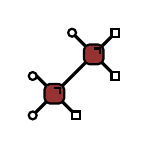
\begin{tikzpicture}[baseline=(current  bounding  box.center), scale=0.5]
\Wgatedagger{-0.5}{-0.5}
\Wgatedagger{0.5}{0.5}
\MYsquare{1.05}{1.05}
\MYsquare{1.05}{-0.05}
\MYsquare{0.05}{-1.05}
\MYcircle{-0.05}{1.05}
\MYcircle{-1.05}{-0.05}
\MYcircle{-1.05}{-1.05}
\end{tikzpicture}
.
\end{equation}The R.H.S. is just the first term of $\mathrm{Tr}B^{\dagger}B$. Similarly,
one can prove that the rest terms of $\mathrm{Tr}A^{\dagger}A$ and
$\mathrm{Tr}B^{\dagger}B$ agree with each other one by one. Eq. (\ref{eq:2ndfig})
will play an important role when calculating the spatio-temporary
correlation function.

\subsection{IRF case (interaction)}

\subsection{Third Hierarchy\label{subsec:Third-Hierarchy}}

Following the idea in subsection \ref{subsec:Second-Hierarchy}, we
can define the condition of $3_{\mathrm{rd}}$ Hierarchy dual as \begin{equation}
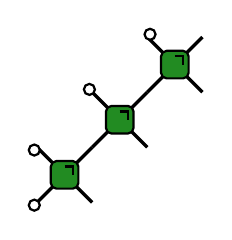
\begin{tikzpicture}[baseline=(current  bounding  box.center), scale=0.7]
\Wgategreen{0.5}{0.5}
\Wgategreen{-0.5}{-0.5}
\MYcircle{-0.05}{1.05}
\MYcircle{-1.05}{-0.05}
\MYcircle{-1.05}{-1.05}
\Wgategreen{1.5}{1.5}
\MYcircle{1.05}{2.05}
\end{tikzpicture}
=
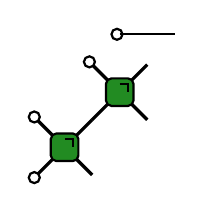
\begin{tikzpicture}[baseline=(current  bounding  box.center), scale=0.7]
\Wgategreen{-0.5}{-0.5}
\Wgategreen{0.5}{0.5}
\MYcircle{-0.05}{1.05}
\MYcircle{-1.05}{0.05}
\MYcircle{-1.05}{-1.05}
\MYcircle{0.45}{1.55}
\draw[thick] (0.5,1.55)--(1.5,1.55);
\end{tikzpicture}
.
\end{equation}Also, it is immediately seen that a gate is $2_{\mathrm{nd}}$ Hierarchy
dual must be $3_{\mathrm{rd}}$ Hierarchy dual. We are also interested
in the case which is only $3_{\mathrm{rd}}$ Hierarchy dual but not
$2_{\mathrm{nd}}$, denoting as $\overline{3}_{\mathrm{rd}}=3_{\mathrm{rd}}-2_{\mathrm{nd}}$.
One example in $\overline{3}_{\mathrm{rd}}$ is Controlled-Z gate.
A fully parametrization in qubit case with $U=v_{1}\otimes v_{2}e^{i(J_{x}\sigma_{x}\sigma_{x}+J_{y}\sigma_{y}\sigma_{y}+J_{z}\sigma_{z}\sigma_{z})}$
is $J_{x}=J_{y}=0$ and $v_{1},v_{2}$ either Pauli matrix in the
$x-y$ plane or diagonal matrix in $z$ basis. Our parametrization
(\textcolor{blue}{here a hyperlink in the future}) can also be applied
here, see SUPPLEMENTAL MATERIAL(citation) for the algebraic equation
for $\theta_{p,q}$. An example is $\theta_{p,q}=\omega^{p^{2}}$
with $v_{1},v_{2}=I_{D}$.

\section{Applications}

In this section, we discuss the physical application of $2_{\mathrm{nd}}$
Hierarchy dual in spatio-temporal correlation functions and quantum
quenches. When properly, we also briefly mention the result for $3_{\mathrm{rd}}$
Hierarchy dual.

\subsection{Spatio-temporal correlations}

In this subsection, we discuss the spatio-temporal correlation functions,
sometimes known as OTOC. The spatio-temporal correlation function
is defined in Heisenberg picture as 
\begin{equation}
C_{ij}(t)=\langle a_{i}(t)b_{j}\rangle=\mathrm{Tr}\left(a_{i}Ub_{j}U^{\dagger}\right),\label{eq:definitionofcorrelationfunction}
\end{equation}
where we take the temperature to be infinity. Since the propagation
of an identity operator is trivial, we further require that $a_{i},b_{j}$
to be both traceless. The correlations in the folded picture are graphically
expressed as \begin{align}
&\braket{a_i(t) b_j}=
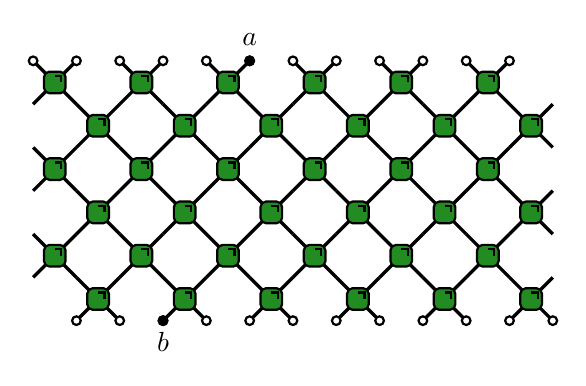
\begin{tikzpicture}[baseline=(current bounding box.center), scale=0.55]
\foreach \jj[evaluate=\jj as \j using -2*(ceil(\jj/2)-\jj/2)] in {0,...,5}
\foreach \i in {1,...,6}
{\Wgategreen{2*\i+\j}{\jj}}
\foreach \i in {2,...,13}{
\MYcircle{\i-.5}{-0.5}
\MYcircle{\i-1.5}{6-0.5}
}
\MYcircleB{3.5}{-.5}
\MYcircleB{5.5}{6-.5}
\Text[x=3.5,y=-1.0]{$b$}
\Text[x=5.5,y=6.0]{$a$}
\end{tikzpicture}\, . \label{eq:Corr1}
\end{align}First, with time unitarity, we can simplify the circuit from the bottom
and top. The result is

\begin{align}
&\braket{a_i(t) b_j}=
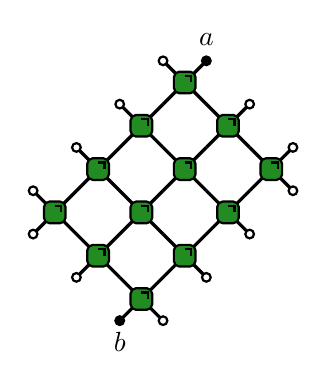
\begin{tikzpicture}[baseline=(current bounding box.center), scale=0.55]
\Wgategreen{3}{0}
\Wgategreen{2}{1}
\Wgategreen{4}{1}
\Wgategreen{1}{2}
\Wgategreen{3}{2}
\Wgategreen{5}{2} 
\Wgategreen{2}{3}
\Wgategreen{4}{3}
\Wgategreen{6}{3}
\Wgategreen{3}{4} 
\Wgategreen{5}{4}
\Wgategreen{4}{5}
\MYcircle{1.5}{0.5}
\MYcircle{0.5}{1.5}
\foreach \i in {1,...,4}
{\MYcircle{2.5+\i}{\i-1.5}}
\foreach \i in {1,...,4}
{
\MYcircle{4.5-\i}{6.5-\i}
}
\MYcircle{5.5}{4.5}
\MYcircle{6.5}{3.5}
\MYcircleB{2.5}{-.5}
\MYcircleB{4.5}{6-.5}
\Text[x=2.5,y=-1.0]{$b$}
\Text[x=4.5,y=6.0]{$a$}
\end{tikzpicture}\, . 
\end{align}

Now we can apply Eq. (\ref{eq2:bottomtotop}) to simplify the circuit
as 

\begin{align}
&\braket{a_i(t) b_j}=
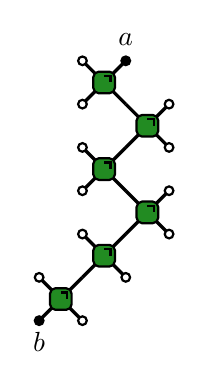
\begin{tikzpicture}[baseline=(current bounding box.center), scale=0.55]
\Wgategreen{4}{5}
\Wgategreen{5}{4}
\Wgategreen{4}{3}
\foreach \i in {1,2,3}
{\Wgategreen{2+\i}{\i-1}}
\foreach \i in {1,...,5}
{
\MYcircle{3.5}{\i+0.5}
}
\foreach \i in {1,2,3}
{\MYcircle{5.5}{1.5+\i}}
\MYcircle{2.5}{0.5}
\foreach \i in {1,2,3}
{\MYcircle{2.5+\i}{\i-1.5}}
\MYcircleB{2.5}{-.5}
\MYcircleB{4.5}{6-.5}
\Text[x=2.5,y=-1.0]{$b$}
\Text[x=4.5,y=6.0]{$a$}
\end{tikzpicture}\, .
\end{align}At last, we can apply Eq. (\ref{eq:2ndfig}) to the corner of the
path, which brings us\begin{align}
&\braket{a_i(t) b_j}=
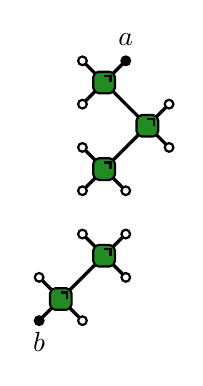
\begin{tikzpicture}[baseline=(current bounding box.center), scale=0.55]
\Wgategreen{4}{5}
\Wgategreen{5}{4}
\Wgategreen{4}{3}
\foreach \i in {1,2}
{\Wgategreen{2+\i}{\i-1}}
\foreach \i in {1,...,5}
{
\MYcircle{3.5}{\i+0.5}
}
\foreach \i in {2,3}
{\MYcircle{5.5}{1.5+\i}}
\MYcircle{2.5}{0.5}
\foreach \i in {1}
{\MYcircle{2.5+\i}{\i-1.5}}
\foreach \i in {1,2,3}
{\MYcircle{4.5}{\i-0.5}}
\MYcircleB{2.5}{-.5}
\MYcircleB{4.5}{6-.5}
\Text[x=2.5,y=-1.0]{$b$}
\Text[x=4.5,y=6.0]{$a$}
\end{tikzpicture}\, .
\end{align}This correlator will vanish because the discontinuous path will finally
simplify to $\mathrm{\mathrm{Tr}}a_{i}\mathrm{Tr}b_{j}$ and in our
assumptions they are both traceless.

Therefore, the only non-vanishing correlators are either at the light
cone or on the same time line

\begin{equation}
\begin{aligned}
&\braket{a_i(t) b_j}\delta_{i,t+j}=
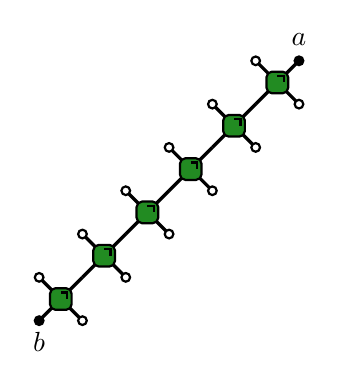
\begin{tikzpicture}[baseline=(current bounding box.center), scale=0.55]
\foreach \i in {0,...,5}
{\Wgategreen{3+\i}{\i}}
\foreach \i in {0,...,5}
{\MYcircle{2.5+\i}{0.5+\i}}
\foreach \i in {0,...,5}
{\MYcircle{3.5+\i}{-0.5+\i}}
\MYcircleB{2.5}{-.5}
\MYcircleB{8.5}{6-.5}
\Text[x=2.5,y=-1.0]{$b$}
\Text[x=8.5,y=6.0]{$a$}
\end{tikzpicture}
,\\
&\braket{a_i(t) b_j}\delta_{i,j}=
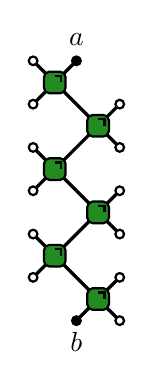
\begin{tikzpicture}[baseline=(current bounding box.center), scale=0.55]
\foreach \i in {0,1,2}
{
\Wgategreen{4}{2*\i}
\Wgategreen{3}{1+2*\i}
\MYcircle{4.5}{2*\i-0.5}
\MYcircle{4.5}{2*\i+0.5}
\MYcircle{2.5}{1.5+2*\i}
\MYcircle{2.5}{0.5+2*\i}
}
\MYcircleB{3.5}{-.5}
\MYcircleB{3.5}{6-.5}
\Text[x=3.5,y=-1.0]{$b$}
\Text[x=3.5,y=6.0]{$a$}
\end{tikzpicture}
.
\end{aligned}
\end{equation}

The above result can also be put into the language of quantum channels.
Here we define four channels

\begin{widetext}
\begin{equation}
\epsilon_L(b)=
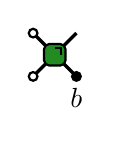
\begin{tikzpicture}[baseline=(current bounding box.center), scale=0.55]
\Wgategreen{0}{0}
\MYcircle{-0.5}{-0.5}
\MYcircle{-0.5}{0.5}
\MYcircleB{0.5}{-0.5}
\Text[x=0.5,y=-1]{$b$}
\end{tikzpicture}
,
\qquad
\epsilon_R(b)=
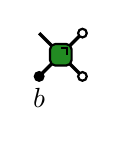
\begin{tikzpicture}[baseline=(current bounding box.center), scale=0.55]
\Wgategreen{0}{0}
\MYcircle{0.5}{-0.5}
\MYcircle{0.5}{0.5}
\MYcircleB{-0.5}{-0.5}
\Text[x=-0.5,y=-1]{$b$}
\end{tikzpicture}
,
\qquad
M_L(b)=
\begin{tikzpicture}[baseline=(current bounding box.center), scale=0.55]
\Wgategreen{0}{0}
\MYcircle{0.5}{-0.5}
\MYcircle{-0.5}{0.5}
\MYcircleB{-0.5}{-0.5}
\Text[x=-0.5,y=-1]{$b$}
\end{tikzpicture}
,
\qquad
M_R(b)=
\begin{tikzpicture}[baseline=(current bounding box.center), scale=0.55]
\Wgategreen{0}{0}
\MYcircle{-0.5}{-0.5}
\MYcircle{0.5}{0.5}
\MYcircleB{0.5}{-0.5}
\Text[x=0.5,y=-1]{$b$}
\end{tikzpicture}
.
\end{equation}
\end{widetext}

With these four channels, the correlation functions can be expressed
as in a compact way. Here for simplicity, we assume that $j$ is an
integer. The very similar argument can be put to the case where $j$
is a half integer.
\begin{equation}
C_{ij}(t)=\begin{cases}
\mathrm{Tr}\left(aM_{L}^{2(i-j)}(b)\right) & t=i-j\\
\mathrm{Tr}\left(a\epsilon_{R}^{\kappa}(\epsilon_{L}\epsilon_{R})^{\lfloor\frac{t}{2}\rfloor}(b)\right) & i=j,t=\mathbb{Z}+\frac{k}{2}\\
0 & \mathrm{others}
\end{cases}\label{eq:expression_CF_1site}
\end{equation}
The behavior exhibited by this correlator is markedly distinct from
that observed in the dual unitary case (citation), wherein a non-zero
value exclusively emerges at the light cone. In contrast, the $2_{\mathrm{n}}$
Hierarchy dual reveals an additional non-vanishing direction present
along the time axis. In the case of qubits, it can be demonstrated
that the channels $\epsilon_{L}$ and $\epsilon_{R}$ are reduced
to the total depolarization channel, leading to the vanishing of correlators
along the light cone. Moreover, after conducting thorough algebraic
calculations, the correlators along the same time line will vanish
precisely after a half step. However, examples for non-vanishing correlators
across all three directions and at all times have been identified
in higher dimensions $D>2$. For instance, utilizing the parametrization
methods, a family with $D=4k+2$, $k\in\mathbb{N}^{+}$ and $\theta_{p,q}=\omega^{\frac{Dpq}{2}}$
can be observed.

If the gate is $\overline{3}_{\mathrm{rd}}$ Hierarchy, the correlation
function will be reduced to 

\begin{equation}
C_{ij}(t)=
\begin{tikzpicture}[baseline=(current bounding box.center), scale=0.55]
\foreach \i in {0,...,5}
{\Wgategreen{0}{2*\i}}
\foreach \i in {0,...,5}
{
\Wgategreen{1}{1+2*\i}
\MYcircle{-2.5}{1.5+\i}
}
\foreach \i in {0,...,4}
{\Wgategreen{-1}{1+2*\i}}
\foreach \i in {0,...,3}
{\Wgategreen{2}{4+2*\i}}
\foreach \i in {0,1,2}
{
\Wgategreen{-2}{2+2*\i}
\MYcircle{-1.5}{7.5+\i}
\MYcircle{1.5}{0.5+\i}
\MYcircle{2.5}{3.5+\i}
\MYcircle{2.5}{8.5+\i}
}
\Wgategreen{3}{7}
\MYcircle{0.5}{-0.5}
\MYcircle{3.5}{6.5}
\MYcircle{3.5}{7.5}
\MYcircle{1.5}{11.5}
\MYcircle{-0.5}{10.5}
\MYcircleB{-0.5}{-0.5}
\MYcircleB{0.5}{11.5}
\Text[x=-0.5,y=-1] {$b$};
\Text[x=.5,y=12] {$a$};
\end{tikzpicture}
.
\end{equation}

This correlator will not vanish inside the entire light cone and there
is no closed expression for it with scaling polynomial in system size.
However, the Hierarchy dual condition can still slower the velocity
of the light cone. In general , for a $k_{\mathrm{th}}$ Hierarchy
dual circuit, the light cone velocity will be suppressed to $\frac{k-2}{k}$.
 

\subsection{Bigger supports and higher orders}

In contrast to earlier studies that focused on correlators supported
on a single site, examining multi-site support may reveal more complex
underlying physics. Specifically, for correlators supported on two
nearest-neighbor sites, the behavior is akin to that described in
Eq. (\ref{eq:expression_CF_1site}), where correlation functions arise
exclusively in three directions. Notably, these correlation functions
do not vanish over time for the qubit case, unlike the operator supported
on a single site.\begin{equation}
\begin{aligned}
&\braket{a_i(t) b_j}\delta_{i,t+j}=
\begin{tikzpicture}[baseline=(current bounding box.center), scale=0.55]
\foreach \i in {1,...,5}
{\Wgategreen{3+\i}{\i}}
\foreach \i in {1,...,5}
{\MYcircle{2.5+\i}{0.5+\i}}
\foreach \i in {1,...,5}
{\MYcircle{3.5+\i}{-0.5+\i}}
\MYsquareB{3.5}{0.5}
\MYsquareB{8.5}{5.5}
\Text[x=3.5,y=-.15]{$b$}
\Text[x=8.5,y=6.15]{$a$}
\end{tikzpicture}
,\\
&\braket{a_i(t) b_j}\delta_{i,j}=
\begin{tikzpicture}[baseline=(current bounding box.center), scale=0.55]
\foreach \i in {1,2}
{
\Wgategreen{4}{2*\i}
\Wgategreen{3}{1+2*\i}
\Wgategreen{5}{1+2*\i}
\MYcircle{5.5}{1.5+2*\i}
\MYcircle{5.5}{0.5+2*\i}
\MYcircle{2.5}{1.5+2*\i}
\MYcircle{2.5}{0.5+2*\i}
}
\Wgategreen{3}{1}
\Wgategreen{5}{1}
\MYcircle{5.5}{1.5}
\MYcircle{5.5}{0.5}
\MYcircle{2.5}{1.5}
\MYcircle{2.5}{0.5}
\MYsquareB{4}{0}
\draw[very thick] (4.25,0.25) -- (4.5,0.5);
\draw[very thick] (3.75,0.25) -- (3.5,0.5);
\MYsquareB{4}{6}
\draw[very thick] (3.75,5.75) -- (3.5,5.5);
\draw[very thick] (4.25,5.75) -- (4.5,5.5);
\Text[x=4,y=-0.75]{$b$}
\Text[x=4,y=6.75]{$a$}
\end{tikzpicture}
,
\end{aligned}
\end{equation}where \begin{tikzpicture}[baseline=(current bounding box.center), scale=0.55]
\MYsquareB{4}{0}
\end{tikzpicture} represents the operator acting on nearest neighbor two sites. In
Fig. (\ref{Correlation_func_sup2}), we draw the correlation function
for the operator supporting on the nearest neighbor two sites. It
is obvious from the figure that the correlation function nonvanishes
only along three directions.

\begin{figure}
\includegraphics[width=0.9\columnwidth]{Figs/correlation_function_support2}

This figure shows the correlation function for operators supporting
on two sites. The gate is chosen as a $\overline{2}_{\mathrm{nd}}$
Hierarchy dual with $D=6$ and parametrization $\theta_{p,q}=\omega^{3pq}$
and $a_{i}=b_{j}=h$, where $h$ is a random Hermitian matrix satisfying
the normalization condition $\mathrm{Tr}h=0,\mathrm{Tr}h^{2}=1$.
The time $t$ and location $i$ are defined in Eq. (\ref{eq:definitionofcorrelationfunction}).
$j$ is fixed to be $20$. Here the location of a $2-$site operator
is defined as the location of its left end. The deeper the color is,
the larger the absolute value of the correlation function is. Another
notice is that this correlation function will not vanish because in
Hermitian space, the channels associated with our chosen gate have
only eigenvalues $0$ or $1$.

\label{Correlation_func_sup2}
\end{figure}

Superseding the scope of $2-$point correlation functions, $3-$point
correlation functions offer the ability to unveil higher orders of
equilibrium information. They are defined as
\begin{equation}
C_{i,j,k}(t_{1},t_{2})=\langle a_{i}(t_{1})b_{j}(t_{2})c_{k}\rangle.
\end{equation}
In scenarios where $i$ and $j$ exist on the same side of $k$, the
$3-$point correlation function can be expressed as 

\begin{equation}
C_{i,j,k}(t_1,t_2)=
\begin{tikzpicture}[baseline=(current bounding box.center), scale=0.55]
\foreach \i in {0,...,4}
{
\Wgategreen{-\i}{\i}
\MYcircle{-\i-0.5}{\i-0.5}
}
\foreach \i in {0,...,4}
{
\Wgategreen{1-\i}{1+\i}
}
\foreach \i in{0,1,2}
{
\Wgategreen{2-\i}{2+\i}
\MYcircle{2.5-\i}{2.5+\i}
}
\MYcircle{1.5}{0.5}
\MYcircle{2.5}{1.5}
\MYcircle{-4.5}{4.5}
\MYcircle{-2.5}{5.5}
\MYcircle{-1.5}{4.5}
\MYcircleB{0.5}{-0.5}
\MYcircleB{-3.5}{5.5}
\MYcircleB{-0.5}{4.5}
\Text[x=0.5,y=-1]{$c$};
\Text[x=-3.5,y=6]{$a$};
\Text[x=-0.5,y=5]{$b$};
\end{tikzpicture}
.
\end{equation}When associated with the $2_{\mathrm{nd}}$ Hierarchy dual, this correlation
function will vanish for traceless operators.

The $3-$point correlation functions only become non-trivial when
$i$ and $j$ are located on different sides of $k$.\begin{equation}
C_{i,j,k}(t_1,t_2)=
\begin{tikzpicture}[baseline=(current bounding box.center), scale=0.55]
\Wgategreen{1}{5}
\MYcircle{1.5}{5.5}
\foreach \i in {0,...,3}
{
\Wgategreen{0}{2*\i}
\Wgategreen{-1}{1+2*\i}
\Wgategreen{1+\i}{3+\i}
\MYcircle{1.5+\i}{2.5+\i}
\MYcircle{-0.5-\i}{7.5+\i}
}
\foreach \i in {0,1}
{\MYcircle{3.5-\i}{6.5-\i}}
\foreach \i in {0,1,2}
{
\Wgategreen{-2-\i}{8+\i}
\MYcircle{0.5}{\i-0.5}
\MYcircle{-2.5-\i}{7.5+\i}
}
\MYcircle{0.5}{6.5}
\foreach \i in {0,...,6}
{
\MYcircle{-1.5}{.5+\i}
}
\MYcircleB{-0.5}{-0.5}
\MYcircleB{4.5}{6.5}
\MYcircleB{-4.5}{10.5}
\Text[x=-0.5,y=-1] {$c$}
\Text[x=4.5,y=7] {$a$}
\Text[x=-4.5,y=11] {$b$}
\end{tikzpicture}
.
\end{equation}Unlike the $1_{\mathrm{st}}$ Hierarchy dual, the non-trivial correlation
function is found to exist within the light cone.

Nonetheless, despite the fact that the $2_{\mathrm{nd}}$ Hierarchy
dual significantly simplifies the circuit complexities, there are
be not solvable. Specifically, inside the light cone, the computational
complexity is $e^{\mathcal{O}(|(t_{1}-|i|)-(t_{2}-|j|)|)}$.

\subsection{Quantum Quench}

In this subsection, we consider the correlation function after a quench
starting from an initial density matrix $\rho(0)$. Here $\rho(0)$
can be both a pure state or mixed state but allows a local purifying
MPS $\rho_{L}(A)=\mathrm{Tr}_{\gamma_{1},\cdots,\gamma_{L}}\ket{\Psi_{L}(A)}\bra{\Psi_{L}(A)}$
(citation), where
\begin{equation}
\begin{aligned}\ket{\Psi_{L}(A)} & =\\
\sum_{\{i_{k}^{\mathrm{L}},i_{k}^{\mathrm{R}},\gamma_{k}\}} & \mathrm{Tr}\left(A^{(i_{1}^{\mathrm{L}}i_{1}^{\mathrm{R}}\gamma_{1})}\cdots A^{(i_{L}^{\mathrm{L}}i_{L}^{\mathrm{R}}\gamma_{L})}\right)\ket{i_{1}^{\mathrm{L}}i_{1}^{\mathrm{R}}\gamma_{1}\cdots i_{L}^{\mathrm{L}}i_{L}^{\mathrm{R}}\gamma_{L}}
\end{aligned}
\end{equation}
 see (citation). Without statements, the gates in this subsection
are all assumed to be $2_{\mathrm{nd}}$ Hierarchy dual. Graphically,
the density matrix can be expressed as\begin{equation}
\rho_L=\frac{1}{d^L} \;
\begin{tikzpicture}[baseline=(current bounding box.center), scale=0.55]
\draw[very thick] (-1.0 ,0.) -- (3.0,0.);
\rhoO{0}{0}\rhoO{2}{0}
\end{tikzpicture}
=
\begin{tikzpicture}[baseline=(current  bounding  box.center), scale=.7]
\def\dx{0.15}
\def\dy{0.15}
\draw[ thick] (-4.75+.2+\dx,0.+\dy) --(-0.0+0.2+\dx,0.+\dy);
%
\draw[ thick] (-3.75+\dx,0.75+\dy) -- (-3.75+\dx,-0.0+\dy);
\draw[ thick] (-3.25+\dx,0.75+\dy) -- (-3.25+\dx,0.0+\dy);
\draw[ thick, fill=myblue, rounded corners=2pt] (-4+\dx,0.25+\dy) rectangle (-2.5+\dx,-0.25+\dy);
%\draw[thick] (-3.75+\dx,0.15+\dy) -- (-3.75+0.15+\dx,0.15+\dy) -- (-3.75+0.15+\dx,0+\dy);
%----
\draw[ thick] (-1.75+\dx,0.75+\dy) -- (-1.75+\dx,-0.0+\dy);
\draw[ thick] (-1.25+\dx,0.75+\dy) -- (-1.25+\dx,0.0+\dy);
\draw[ thick, fill=myblue, rounded corners=2pt] (-2+\dx,0.25+\dy) rectangle (-0.5+\dx,-0.25+\dy);
\draw[ thick] (-2.75 ,0.25) -- (-2.75,0.25+.2) --(-2.75+\dx,0.25+\dy+.2) --(-2.75+\dx,0.25+\dy);
%Horizontal 
\draw[ thick] (-4.75 ,0.) -- (-.0+.2,0.);
\draw[ thick] (-3.75,0.75) -- (-3.75,-0.0);
\draw[ thick] (-3.25,-0.0) -- (-3.25,0.75);
\draw[ thick, fill=myorange0, rounded corners=2pt] (-4,0.25) rectangle (-2.5,-0.25);
\draw[ thick] (-1.75,0.75) -- (-1.75,-0.0);
\draw[ thick] (-1.25,-0.0) -- (-1.25,0.75);
\draw[ thick, fill=myorange0, rounded corners=2pt] (-2,0.25) rectangle (-0.5,-0.25);
%----
\draw[ thick] (-0.75 ,0.25) -- (-0.75,0.25+.2) --(-0.75+\dx,0.25+\dy+.2) --(-0.75+\dx,0.25+\dy);
%\Text[x=-3.65,y=0.75]{$i^L j^L$}
\end{tikzpicture} \; ,
\end{equation}

The property of initial state is inherited in the time evolution of
$1-$point correlation function defined as 
\begin{equation}
\lim_{L\to\infty}\braket{\psi_{t}^{L}|O_{1}|\psi_{t}^{L}}=\lim_{k\to\infty}\mathrm{tr}(E^{k}(t)E_{O_{1}}(t)E^{k}(t)),
\end{equation}
where $E(t)$ and $E_{O_{1}}(t)$ are appropriate transfer matrices
acting along the transverse time axis

\begin{equation}
\begin{aligned}
\braket{\psi_t^L|O_1|\psi_t^L} & =
\begin{tikzpicture}[baseline=(current bounding box.center), scale=0.55]
\foreach \i in {0,2,4,6}
{\rhoO{\i}{0}}
\draw [very thick] (-0.5,0) -- (6.5,0);
\foreach \i in {1,3,5}
{
\foreach \j in {1,3}
{
\Wgategreen{\i}{\j}
}
}
\foreach \i in {0,2,4,6}
{
\foreach \j in {2,4}
{
\Wgategreen{\i}{\j}
}
}
\foreach \i in {0,1,2,3,5,6,7}
{
\MYcircle{\i-0.5}{4.5}
}
\MYcircleB{3.5}{4.5}
\Text[x=3.5,y=5] {$O_1$};
\end{tikzpicture}
, \\
E(t) & =
\begin{tikzpicture}[baseline=(current bounding box.center), scale=0.55]
\rhoO{0}{0}
\draw [very thick] (-1,0) -- (1,0);
\foreach \j in {1,3}
{
\Wgategreen{-1}{\j}
}
\foreach \j in {2,4}
{
\Wgategreen{0}{\j}
}
\MYcircle{-0.5}{4.5}
\MYcircle{0.5}{4.5}
\end{tikzpicture}
\end{aligned}
.
\end{equation}If the initial state satisfies the following condition

\begin{equation}
\begin{tikzpicture}[baseline=(current bounding box.center), scale=0.55]
\rhoO{0}{0}
\Wgategreen{-1}{1}
\MYcircle{-0.5}{1.5}
\MYcircle{0.5}{0.5}
\MYsquare{0.5}{0}
\end{tikzpicture}
=\frac{1}{D}
\begin{tikzpicture}[baseline=(current bounding box.center), scale=0.55]
\draw[very thick] (-0.5,0) -- (0.5,0);
\Wgategreen{-1}{1}
\MYcircle{-0.5}{1.5}
\MYcircle{-0.5}{0.5}
\MYsquare{0.5}{0}
\end{tikzpicture}
, \label{eq:transfer_condi}
\end{equation}we can find an eigenstate of the transfer matrix with eigenvalue $1$\begin{equation}
E(t)\;
\begin{tikzpicture}[baseline=(current bounding box.center), scale=0.55]
\draw[very thick] (-0.5,0)--(0.5,0);
\MYsquare{0.5}{0}
\foreach \j in {1,3}
{
\Wgategreen{0}{\j}
}
\foreach \j in {1,2,3,4}
{
\MYcircle{0.5}{\j-0.5}
}
\end{tikzpicture}
\;
=
\;
\begin{tikzpicture}[baseline=(current bounding box.center), scale=0.55]
\draw[very thick] (-0.5,0)--(0.5,0);
\MYsquare{0.5}{0}
\foreach \j in {1,3}
{
\Wgategreen{0}{\j}
}
\foreach \j in {1,2,3,4}
{
\MYcircle{0.5}{\j-0.5}
}
\end{tikzpicture}
.
\end{equation}Since $\lim_{L\to\infty}\braket{\psi_{t}^{L}|\psi_{t}^{L}}=1$ due
to the normalization, the largest eigenvalue of the trasnfer matrix
must be $1$ and non-degenerate. Therefore, the $1-$point correlation
function can be analytically calculated with this eigenvector. Eq.
(\ref{eq:transfer_condi}) is also called the $1-$point solvable
condition for $\overline{2}_{\mathrm{nd}}$ Hierarchy dual.

It should be noted that if the initial state satisfies the condition$
\begin{tikzpicture}[baseline=(current bounding box.center), scale=0.55]
\rhoO{0}{0}
\MYcircle{0.5}{0.5}
\MYsquare{0.5}{0}
\end{tikzpicture}
\;
=
\begin{tikzpicture}[baseline=(current bounding box.center), scale=0.55]
\draw[very thick] (-0.5,0) -- (0.5,0);
\draw[very thick] (-0.5,0.5) -- (0.5,0.5);
\MYcircle{0.5}{0.5}
\MYsquare{0.5}{0}
\end{tikzpicture}
\,
,
$Eq. (\ref{eq:transfer_condi}) is automatically followed. This means
that we found a larger solvable class than the one in (citation).

The $2-$point correlation functions after a quench (citation) is
diagrammatically described as

\begin{align}\label{eq:quench2}
&C_{ij}(t) = 
\begin{tikzpicture}[baseline=(current  bounding  box.center), scale=0.55]
\foreach \i in {0,...,1}
{
\Wgategreen{-2}{0+2*\i}
\Wgategreen{0}{0+2*\i}
\Wgategreen{2}{0+2*\i}
\Wgategreen{4}{0+2*\i}
\Wgategreen{6}{0+2*\i}
%\Wgategreen{8}{0+2*\i}
\Wgategreen{-1}{1+2*\i}
\Wgategreen{1}{1+2*\i}
\Wgategreen{3}{1+2*\i}
\Wgategreen{5}{1+2*\i}
\Wgategreen{7}{1+2*\i}
%\Wgategreen{9}{1+2*\i}
}
\draw[very thick] (-2.25,-1) -- (7.5,-1);
\foreach \i in {2.5,4.5,6.5,8.5,10.5}
{\rhoO{-3.5+\i}{-1}}
%  
\foreach \i in {-1,...,8}
{ 
\draw[thick, fill=white] (\i-0.5,4-0.5) circle (0.1cm);
}
\MYcircleB{7.5}{3.5}
\MYcircleB{-1.5}{3.5}
\Text[x=-1.5,y=4.0]{$a$}
\Text[x=7.5,y=4.0]{$b$}
\end{tikzpicture}
.
\end{align} 

Next, we use time unitarity, which results in two backward propagating
light cones originating from the operators, connected by the transfer
matrix 

\begin{widetext}
\begin{align}
C_{ij}(t)=
\begin{tikzpicture}[baseline=(current  bounding  box.center), scale=0.55]
\Wgategreen{-4}{0}
\Wgategreen{-2}{0}
\Wgategreen{0}{0}
\Wgategreen{2}{0}
\Wgategreen{4}{0}
\Wgategreen{6}{0}
\Wgategreen{8}{0}
\Wgategreen{10}{0}
%
\Wgategreen{-1}{3}
\Wgategreen{7}{3}
\Wgategreen{-2}{2}
\Wgategreen{0}{2}
\Wgategreen{6}{2}
\Wgategreen{8}{2}
\Wgategreen{-3}{1}
\Wgategreen{-1}{1}
\Wgategreen{1}{1}
\Wgategreen{5}{1}
\Wgategreen{7}{1}
\Wgategreen{9}{1}
%
\draw[very thick] (-6.5,-1) -- (13.5,-1);
\draw[very thick,dotted] (-8.5,-1) -- (-6.5,-1);
\draw[very thick,dotted] (13.5,-1) -- (14.5,-1);
\foreach \i in {-3.5,-1.5,0.5,2.5,4.5,6.5,8.5,10.5,12.5,14.5,16.5}
{ \rhoO{-3.5+\i}{-1} }
%
\foreach \i in {0,...,3}
{
\MYcircle{\i-.5}{3.5-\i}
\MYcircle{\i+4-.5}{0.5+\i}
\MYcircle{\i-.5+8}{3.5-\i}
\MYcircle{\i-4-.5}{0.5+\i}
}
\MYcircle{-5.5}{-.5}  
\MYcircle{-6.5}{-.5} 
\MYcircle{-7.5}{-.5}
\MYcircle{11.5}{-.5}  
\MYcircle{12.5}{-.5}  
\MYcircle{13.5}{-.5} 
\MYcircleB{7.5}{3.5} 
\MYcircleB{-1.5}{3.5}
\Text[x=-1.5,y=4.0]{$a$}
\Text[x=7.5,y=4.0]{$b$}
\end{tikzpicture}.
\label{eq:quench4}
\end{align}
.
\end{widetext} In principle, the number of the transfer matrices in the middle $E(0)$
depends on the separation as $j-i-(t_{1}+t_{2})+\frac{1}{2}$. The
solvability condition for the this correlation function is defined
as

\begin{equation}
\begin{tikzpicture}[baseline=(current  bounding  box.center), scale=0.55]
\rhoO{0}{0}
\MYsquare{0.5}{0}
\MYcircle{0.5}{0.5}
\end{tikzpicture}
=
\begin{tikzpicture}[baseline=(current  bounding  box.center), scale=0.6]
\draw[very thick] (-0.5,0) -- (0.5,0);
\draw[very thick] (-0.5,0.5) -- (0.5,0.5);
\MYsquare{0.5}{0}
\MYcircle{0.5}{0.5}
\end{tikzpicture}\;
;
\qquad
\begin{tikzpicture}[baseline=(current  bounding  box.center), scale=0.6]
\rhoO{0}{0}
\MYsquare{0.5}{0}
\Wgategreen{1}{1}
\MYcircle{1.5}{1.5}
\MYcircle{1.5}{0.5}
\end{tikzpicture}
=
\begin{tikzpicture}[baseline=(current  bounding  box.center), scale=0.55]
\draw[very thick] (-0.5,0) -- (0.5,0);
\draw[very thick] (-0.5,0.5) -- (0.5,0.5);
\MYsquare{0.5}{0}
\MYcircle{0.5}{0.5}
\MYcircle{0.5}{1.5}
\draw[very thick] (-0.5,1.5) -- (0.5,1.5);
\end{tikzpicture}\;
.\label{eq:solvable2points}
\end{equation}Following the same argument in (citation), we can always replace \begin{tikzpicture}[baseline=(current  bounding  box.center), scale=0.55]
\draw[very thick] (-0.5,0) -- (0.5,0);
\MYsquare{0.5}{0}
\end{tikzpicture} by \begin{tikzpicture}[baseline=(current  bounding  box.center), scale=0.55]
\draw[very thick] (-0.5,0) -- (0.5,0);
\MYcircle{0.5}{0}
\end{tikzpicture}. 

Substituting \ref{eq:solvable2points} into \ref{eq:quench4}, we
have a very simplified expression for the correlation function\begin{equation}
C_{ij}(t)=
\begin{tikzpicture}[baseline=(current  bounding  box.center), scale=0.55]
\rhoO{0}{0}
\foreach \i in {1,2,3,4}
{
\Wgategreen{\i}{\i}
\Wgategreen{-\i}{\i}
\MYcircle{\i-0.5}{\i+0.5}
\MYcircle{\i+0.5}{\i-0.5}
\MYcircle{0.5-\i}{\i+0.5}
\MYcircle{-0.5-\i}{\i-0.5}
}
\MYcircle{0.5}{0}
\MYcircle{-0.5}{0}
\MYcircleB{4.5}{4.5}
\MYcircleB{-4.5}{4.5}
\Text[x=4.5,y=5]{$b$}
\Text[x=-4.5,y=5]{$a$}
\end{tikzpicture}
\end{equation}

on the other hand, if the separation $j-i$ is shorter than $t_{1}+t_{2}$,
the correlation function will vanish for traceless operators.

Eq. (\ref{eq:solvable2points}) can be put into an algebraic form.
If we define the operator
\begin{equation}
K^{(\gamma)\dagger}:=\sum_{i^{\mathrm{L}}j^{\mathrm{R}}}A^{(i^{\mathrm{L}}j^{\mathrm{R}}\gamma)}\otimes|i^{\mathrm{L}}\rangle\langle j^{\mathrm{R}}|,
\end{equation}
the solvable condition can be written as
\begin{equation}
\begin{aligned}\sum_{\gamma}K_{\gamma}^{\dagger}K_{\gamma} & =\frac{I_{d\chi}}{d};\\
\sum_{\gamma}I_{d}\otimes K_{\gamma}^{\dagger}(\tilde{U^{\dagger}}\tilde{U}\otimes I_{\chi})K_{\gamma}\otimes I_{d} & =\frac{I_{d^{2}\chi}}{d}.
\end{aligned}
\end{equation}
Specifically, if the initial state is a pure state, namely no summation
over $\gamma$, the first equation will imply that $K$ is proportional
to a unitary operator, leading to the fact that $U$ is $1_{\mathrm{st}}$
Hierarchy dual from the second equation. Therefore, the solvable initial
state for $\overline{2}_{\mathrm{nd}}$ can only be mixed state. For
example, if we choose $U=\mathrm{CNOT}$ and the bond dimension for
MPS to be $1$, a nontrivial solution is $K_{0}=\frac{I}{2\sqrt{2}},K_{1}=\frac{\sigma_{Y}}{2\sqrt{2}}$.
Here $\sigma_{Y}=\begin{pmatrix}0 & -i\\
i & 0
\end{pmatrix}$.

At last, we mentioned that a similar method for dealing $2-$point
correlation functions can also be applied to $1-$point correlation
function and the same solvable condition (\ref{eq:transfer_condi})
follows.

\section{Conclusion and Perspectives}

It is worthy mentioning that though in the paper, our main focus is
on the translational invariance one, the result here does not rely
on this property. The ideas here can be directly generalized to the
case where some inhomogeneous or randomness is included in space and/or
time.
\end{document}
